\begin{problem}
\textbf{\textsc{Con lắc cơ giới 1}}
Một con lắc được làm từ một thanh không trọng lượng có chiều dài $l=0.5000\;\mathrm{m}$ và một chất điểm $m=15.00\;\mathrm{kg}$ treo ở một đầu. Góc giữa thanh và phương thẳng đứng là $\theta$. Một động cơ gắn vào điểm xoay cung cấp một mô-men xoắn. Giá trị lớn nhất của moment xoắn này phụ thuộc vào góc và được cho bởi $\tau (\theta)=\frac{1+\cos\theta}{2} \tau_0$ for $0\leq \theta \leq 90^{\circ}$.

\begin{figure}[h]
    \centering
    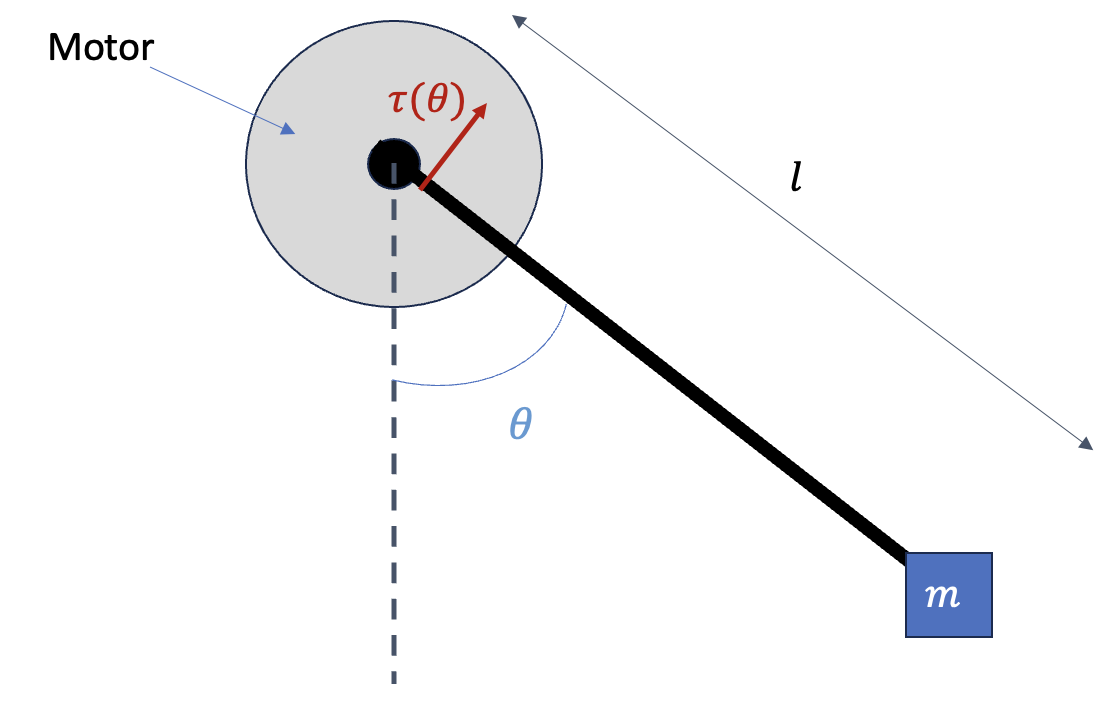
\includegraphics[width=0.5\linewidth]{problems/figures/mot_pend.png}
    \caption{Con lắc cơ giới.}
    \label{fig:enter-label}
\end{figure}

Con lắc ban đầu được cho một vận tốc góc nhỏ theo chiều ngược chiều kim đồng hồ và ở $\theta = 0$. Khối lượng rất nhạy cảm và không thể chịu được tốc độ cao. Do đó, giả sử động cơ luôn cung cấp đủ momemt xoắn để khối lượng di chuyển với tốc độ hầu như không thay đổi. Giá trị nhỏ nhất của $\tau_0$ cần thiết để con lắc cuối cùng đạt đến $\theta=90^{\circ}$ là bao nhiêu?


\end{problem}
